% !TEX program = pdflatex
% University of Malakand Thesis Style (adapted) – with Magazine‑Style Injector
\documentclass[12pt, a4paper, oneside]{book}

% ===== PACKAGES (original + injector extras) =====
\usepackage[utf8]{inputenc}
\usepackage[T1]{fontenc}
% Font: Times-like fallback (unchanged)
\IfFileExists{tgtermes.sty}{%
  \usepackage{tgtermes}%
  \IfFileExists{newtxmath.sty}{\usepackage{newtxmath}}{}%
}{%
  \IfFileExists{newtxtext.sty}{%
    \IfFileExists{xpatch.sty}{%
      \usepackage{newtxtext}%
      \usepackage{newtxmath}%
    }{%
      \usepackage{lmodern}%
      \typeout{WARNING: Times-like font packages missing. Using Latin Modern.}%
    }%
  }{%
    \usepackage{lmodern}%
  }%
}
\usepackage{geometry}          % Margins
\usepackage{xcolor}            % Colours
\usepackage{tikz}              % Diagrams
\usetikzlibrary{positioning,arrows.meta}
\usepackage{pgfplots}          % Charts
\pgfplotsset{compat=1.18}
\usepackage{fancyhdr}          % Footer page numbers
\usepackage{multicol}          % Two‑column lists
\usepackage{amsmath, amssymb}  % Math
\usepackage{graphicx}          % Images
\usepackage{booktabs}          % Professional tables (already present)
\usepackage{array}             % Table columns
\usepackage{colortbl}          % Row/column colours
\usepackage{setspace}          % 1.5 line spacing
\usepackage{microtype}         % Better typography
\usepackage{hyperref}          % Hyperlinks
\usepackage{bookmark}          % PDF bookmarks
\usepackage{ragged2e}          % Slightly nicer justification
\usepackage{caption}           % Custom caption formatting

% ==== NEW PACKAGES FOR MAGAZINE STYLE (injector) ====
\usepackage[most]{tcolorbox}   % modern boxes
\usepackage{titlesec}          % stylish section headings
\usepackage{listings}          % code snippets

% ===== MARGINS (University of Malakand) – UNCHANGED =====
\geometry{
  a4paper,
  left=1.5in,
  right=1in,
  top=1in,
  bottom=1in,
  includeheadfoot
}

% ===== COLOURS (original + injector uses AccentBlue) =====
\definecolor{DeepObsidian}{HTML}{111111}
\definecolor{LightGray}{gray}{0.96}
\definecolor{AccentBlue}{HTML}{0B5394}
\definecolor{CyberCyan}{HTML}{0B5394}
\definecolor{ElectricIndigo}{HTML}{3C78D8}
\definecolor{TableRowOdd}{gray}{0.98}
\definecolor{CodeBg}{gray}{0.95}

% ===== TYPOGRAPHY (unchanged) =====
\microtypesetup{protrusion=true, expansion=true}
\renewcommand{\familydefault}{\rmdefault}
\setlength{\parindent}{1.2em}
\setlength{\parskip}{0.6ex plus 0.2ex minus 0.1ex}

% ===== PAGE NUMBERS (bottom-right) – UNCHANGED =====
\pagestyle{fancy}
\fancyhf{}
\renewcommand{\headrulewidth}{0pt}
\renewcommand{\footrulewidth}{0pt}
\fancyfoot[R]{\thepage}
\setlength{\footskip}{0.75in}
\fancypagestyle{plain}{%
  \fancyhf{}
  \renewcommand{\headrulewidth}{0pt}
  \fancyfoot[R]{\thepage}
}

% ===== ORIGINAL KEY INSIGHT BOX (kept for compatibility) =====
\newenvironment{keyinsight}{%
  \par\medskip\noindent
  \begin{center}
    \begin{minipage}{0.92\textwidth}
      \colorbox{LightGray}{%
        \parbox{\dimexpr\linewidth-2\fboxsep\relax}{%
          \small\textbf{Key Insight:}\quad\ignorespaces
        }%
      }%
    \end{minipage}
  \end{center}
  \small
}{%
  \par\medskip
}

% ===== HYPERREF (unchanged) =====
\hypersetup{
  colorlinks=true,
  linkcolor=AccentBlue,
  urlcolor=AccentBlue,
  citecolor=AccentBlue
}

% ===== CUSTOM COMMANDS (unchanged) =====
\newcommand{\thesistitle}{Cardiovascular Disease Prediction Using Machine Learning}
\newcommand{\thesisauthor}{Sajjad Alam}
\newcommand{\thesisdegree}{Bachelor of Science (Statistics)}
\newcommand{\thesisdept}{Department of Statistics}
\newcommand{\thesisuni}{University of Malakand}
\newcommand{\thesisyear}{2026}

% ===== CAPTION STYLE (unchanged) =====
\captionsetup{font=small, labelfont=bf, textfont=it, color=AccentBlue}

% ===== MAGAZINE‑STYLE INJECTOR (safe for university rules) =====
% 1. Modern tcolorbox for key insights / summaries
\newtcolorbox{modernbox}[1]{
  colback=AccentBlue!5!white,
  colframe=AccentBlue!80!black,
  fonttitle=\bfseries\sffamily,
  title=#1,
  arc=2mm,
  boxrule=1pt,
  left=10pt,
  right=10pt,
  top=10pt,
  bottom=10pt,
  enhanced,
  drop shadow        % lighter than shadow=...; remove if printer complains
}

% 2. Code listings styling (for your Python/ML scripts)
\lstset{
  backgroundcolor=\color{LightGray},
  basicstyle=\small\ttfamily,
  keywordstyle=\color{AccentBlue},
  commentstyle=\color{green!50!black},
  stringstyle=\color{orange},
  frame=single,
  breaklines=true,
  captionpos=b,
  frameround=fttt,
  rulecolor=\color{AccentBlue!30}
}

% 3. Magazine-style section headings (does not change numbering or spacing)
\titleformat{\section}
  {\color{AccentBlue}\normalfont\Large\bfseries\sffamily}
  {\thesection}{1em}{}
  [{\titlerule[0.5pt]}]

% ===== DOCUMENT =====
\begin{document}
\onehalfspacing

% ---- FRONTMATTER (Roman numerals) ----
\frontmatter

% ----- TITLE PAGE (beautified, still university pattern) -----
\begin{titlepage}
  \thispagestyle{empty}
  \centering
  \vspace*{1cm}
  {\bfseries\Large\MakeUppercase{Thesis}\par}
  \vspace{1cm}
  {\bfseries\huge\MakeUppercase{\thesistitle}\par}
  \vspace{1.5cm}
  {\large A thesis submitted in partial fulfillment of the requirements for the degree of\par}
  \vspace{0.5cm}
  {\bfseries\Large \thesisdegree\par}
  \vspace{1.2cm}
  {\large By\par}
  \vspace{0.3cm}
  {\bfseries\Large\MakeUppercase{\thesisauthor}\par}
  \vspace{1.5cm}
  \thesisdept\par
  \vspace{0.2cm}
  \thesisuni\par
  \vspace{1cm}
  {\color{AccentBlue}\rule{0.6\textwidth}{0.5pt}\par}
  \vspace{0.5cm}
  {\bfseries\large \thesisyear\par}
  \vfill
\end{titlepage}

% Start roman page numbering at ii
\pagenumbering{roman}
\setcounter{page}{2}

% ----- DECLARATION (unchanged content) -----
\chapter*{Declaration}
\addcontentsline{toc}{chapter}{Declaration}
I, \thesisauthor, hereby declare that this thesis titled ``\thesistitle'' is my own work and has not been submitted previously for any other degree or professional qualification.
\par\bigskip
Signature:\dotfill\par
Date:\dotfill

% ----- PLAGIARISM UNDERTAKING -----
\chapter*{Plagiarism Undertaking}
\addcontentsline{toc}{chapter}{Plagiarism Undertaking}
I solemnly declare that the research work presented in this thesis is my own work. Any material used from other sources has been properly acknowledged and cited.
\par\bigskip
Signature:\dotfill\par
Date:\dotfill

% ----- SUBMISSION AUTHORIZATION CERTIFICATE -----
\chapter*{Submission Authorization Certificate (For Evaluation)}
\addcontentsline{toc}{chapter}{Submission Authorization Certificate}
Certified that the thesis of \thesisauthor\ entitled ``\thesistitle'' has been reviewed in final form and permission is granted to submit it to \thesisuni\ for evaluation.
\par\bigskip
Supervisor:\dotfill\par
Co-supervisor (if any):\dotfill\par
Chairman:\dotfill

% ----- APPROVAL CERTIFICATE -----
\chapter*{Approval Certificate (For the Award of Degree)}
\addcontentsline{toc}{chapter}{Approval Certificate}
It is certified that the work contained in this thesis entitled ``\thesistitle'' was carried out by \thesisauthor\ under supervision and is adequate in scope and quality for the award of the degree.
\par\bigskip
Supervisor:\dotfill\par
Co-supervisor (if any):\dotfill\par
External Examiner:\dotfill\par
Chairman:\dotfill

% ----- DEDICATION -----
\chapter*{Dedication}
\addcontentsline{toc}{chapter}{Dedication}
\begin{center}
\emph{(Write your dedication here.)}
\end{center}

% ----- ACKNOWLEDGMENTS -----
\chapter*{Acknowledgments}
\addcontentsline{toc}{chapter}{Acknowledgments}
I would like to thank my supervisor, teachers, and family for their guidance and support during this research. I also acknowledge the open-source community for providing high-quality machine learning tools.

% ----- TABLE OF CONTENTS -----
\tableofcontents
\listoffigures
\listoftables

% ----- LIST OF ABBREVIATIONS -----
\chapter*{List of Abbreviations}
\addcontentsline{toc}{chapter}{List of Abbreviations}
\begin{multicols}{2}
\begin{itemize}
\item CVD: Cardiovascular disease
\item BMI: Body mass index
\item ROC: Receiver operating characteristic
\item AUC: Area under the curve
\item SHAP: SHapley Additive exPlanations
\end{itemize}
\end{multicols}

% ----- LIST OF PUBLICATIONS (optional) -----
\chapter*{List of Publications}
\addcontentsline{toc}{chapter}{List of Publications}
\emph{(If any, list your publications here.)}

% ----- ABSTRACT -----
\chapter*{Abstract}
\addcontentsline{toc}{chapter}{Abstract}
This thesis develops a practical machine learning system for predicting cardiovascular disease risk from routinely collected health attributes. Using a structured cardiovascular dataset containing demographic, clinical, and lifestyle features, multiple model families are compared (Logistic Regression, SVM, Random Forest, Neural Network, and gradient boosting). The best-performing models are deployed behind a FastAPI service with a user-friendly web interface. The system returns a probability score, a thresholded decision, and explainability information (SHAP) to highlight key drivers behind each prediction.

% ===== MAINMATTER (Arabic numerals) =====
\mainmatter
\pagenumbering{arabic}

% ==================================================
% THESIS CONTENT (r1_content.tex) – fully preserved
% ==================================================
\chapter{INTRODUCTION}

\section{Background of the Study}

Cardiovascular disease (CVD) remains a major cause of mortality globally and represents a substantial public health burden. Millions of people lose their lives every year due to heart-related diseases like heart failure, coronary artery disease, and stroke, health reports worldwide have claimed. These diseases are often linked with lifestyle risk factors such as an unhealthy diet, inadequate physical activity, smoking, and diabetes, high blood pressure and obesity. It is important Because it can be a very deadly disease and early detection of the disease in order to improve, implementation of necessary treatment options.

Traditional medical diagnosis relies heavily on physicians’ experience, laboratory tests, and clinical guidelines. While these methods are effective, they may sometimes fail to capture complex patterns and hidden relationships within medical data. With the increasing availability of healthcare data and advancements in computing technologies, machine learning has emerged as a powerful approach for analyzing large medical datasets and assisting in disease prediction.

Machine learning algorithms are capable of learning patterns from historical data and making predictions on new, unseen data. In the healthcare domain, these techniques can assist doctors in identifying high-risk patients and supporting early diagnosis. Machine learning models such as Logistic Regression, Random Forest, Support Vector Machine (SVM), and Gradient Boosting have been widely used in medical research for disease prediction tasks.

The cardiovascular disease dataset used in this research contains various medical attributes such as age, gender, blood pressure, cholesterol levels, glucose levels, smoking habits, alcohol consumption, and physical activity. By analyzing these features, machine learning models can identify patterns that may indicate whether a person is likely to develop cardiovascular disease.

The application of machine learning in healthcare has the potential to improve diagnostic accuracy, reduce healthcare costs, and provide decision support to medical professionals. Therefore, developing a reliable cardiovascular disease prediction model is an important research area in modern healthcare analytics.

\section{Problem Statement}

Despite advancements in medical science, cardiovascular disease remains a major cause of mortality across the globe. Early detection and prevention are essential for reducing the impact of heart-related diseases. However, traditional diagnostic methods often depend on manual interpretation of clinical data, which can be time-consuming and prone to human error.

Medical datasets usually contain a large number of variables and complex relationships between them. Traditional statistical models may struggle to accurately identify nonlinear relationships among these risk factors. As a result, there is a growing need for intelligent systems that can analyze large volumes of medical data and provide accurate predictions regarding the likelihood of cardiovascular disease.

Machine learning techniques provide an opportunity to overcome these limitations by automatically learning patterns from data. However, selecting the most appropriate algorithm and evaluating its performance remains a challenge. Therefore, this study aims to develop and evaluate machine learning models for predicting cardiovascular disease using clinical data.

\section{Research Objectives}

The main objective of this research is to develop a machine learning-based model that can accurately predict the risk of cardiovascular disease.

The specific objectives of this study are:

\begin{multicols}{2}
\begin{itemize}
\item To analyze the cardiovascular disease dataset and understand the relationships between different medical attributes.
\item To preprocess and prepare the dataset for machine learning model training.
\item To implement multiple machine learning algorithms for cardiovascular disease prediction.
\item To evaluate the performance of different models using appropriate evaluation metrics.
\item To identify the most important features that contribute to cardiovascular disease prediction.
\end{itemize}
\end{multicols}

\section{Research Questions}

This research aims to answer the following questions:

\begin{multicols}{2}
\begin{itemize}
\item Can machine learning models accurately predict the presence of cardiovascular disease using clinical data?
\item Which machine learning algorithm provides the best prediction performance for this dataset?
\item What are the most significant risk factors contributing to cardiovascular disease?
\end{itemize}
\end{multicols}

\section{Significance of the Study}

This study contributes to the field of healthcare analytics by demonstrating the potential of machine learning techniques for cardiovascular disease prediction. The findings of this research may help healthcare professionals identify high-risk patients at an early stage and take preventive measures.

The proposed model can also serve as a decision support tool that assists doctors in diagnosing cardiovascular disease more efficiently. Furthermore, this research highlights the importance of data-driven approaches in modern healthcare systems and encourages further research in the application of artificial intelligence in medical diagnosis.

\section{Scope of the Study}

This research focuses on the development of machine learning models for predicting cardiovascular disease using a structured medical dataset. The study includes data preprocessing, exploratory data analysis, model training, and performance evaluation.

However, this research is limited to the dataset used in this study and does not include real-time clinical deployment. Future work may focus on integrating the developed model into healthcare systems for real-world applications.

\section{Structure of the Thesis}

This thesis is organized into the following chapters:

Chapter 1 provides an introduction to the research problem, objectives, and significance of the study.

Chapter 2 presents a review of related literature and previous research conducted in the field of cardiovascular disease prediction using machine learning.

Chapter 3 describes the research methodology, including dataset description, data preprocessing, and machine learning techniques used in the study.

Chapter 4 presents the experimental results and discusses the performance of different machine learning models.

Chapter 5 concludes the study and provides recommendations for future research.

\chapter{LITERATURE REVIEW}

\section{Introduction}

Cardiovascular disease (CVD) is a major global health concern and has been the subject of extensive research in the medical and data science communities. With the rapid growth of healthcare data and advancements in computational technologies, machine learning techniques have been increasingly applied in the prediction and diagnosis of cardiovascular diseases. This chapter reviews previous studies and research work related to cardiovascular disease prediction using machine learning methods.

The purpose of this literature review is to analyze existing research, identify commonly used machine learning algorithms, and highlight the strengths and limitations of previous studies. Understanding previous research helps in identifying research gaps and justifying the importance of the proposed study.

\section{Cardiovascular Disease and Risk Factors}

Cardiovascular disease refers to a group of disorders affecting the heart and blood vessels. These conditions include coronary artery disease, heart failure, hypertension, and stroke. Several risk factors contribute to the development of cardiovascular disease, including both controllable and uncontrollable factors.

Common risk factors include age, gender, high blood pressure, high cholesterol levels, diabetes, obesity, smoking, alcohol consumption, and lack of physical activity. According to global health statistics, lifestyle-related factors play a significant role in increasing the risk of cardiovascular disease.

Early identification of these risk factors is essential for preventing serious health complications. Traditionally, healthcare professionals use medical tests and clinical guidelines to assess cardiovascular risk. However, these approaches may not always detect complex relationships between multiple variables.

\section{Machine Learning in Healthcare}

Machine learning is a branch of artificial intelligence that enables computers to learn from data and make predictions without being explicitly programmed. In the healthcare domain, machine learning has been widely used for disease prediction, medical image analysis, drug discovery, and personalized medicine.

Machine learning models can analyze large medical datasets and identify hidden patterns that may not be easily recognized through traditional statistical methods. These models are capable of improving diagnostic accuracy and supporting clinical decision-making.

Several machine learning algorithms have been successfully applied in healthcare research, including logistic regression, decision trees, support vector machines, random forests, and neural networks. These algorithms can classify patients into different risk categories based on their medical attributes.

\section{Previous Studies on Cardiovascular Disease Prediction}

Many researchers have explored the use of machine learning techniques for predicting cardiovascular disease. Different studies have used various datasets and algorithms to develop predictive models.

One study applied logistic regression and decision tree algorithms to predict heart disease using patient clinical data. The results showed that logistic regression provided reliable baseline performance while decision trees helped in understanding the importance of different features.

Another research study utilized support vector machines and random forest algorithms for cardiovascular disease prediction. The findings indicated that ensemble methods such as random forest often achieve higher accuracy due to their ability to combine multiple decision trees and reduce overfitting.

In recent years, gradient boosting algorithms such as XGBoost have gained popularity in predictive modeling. These algorithms improve model performance by combining multiple weak learners into a strong predictive model.

Deep learning approaches have also been explored in cardiovascular disease prediction. Neural networks are capable of learning complex nonlinear relationships within medical data. However, they often require larger datasets and higher computational resources.

\section{Comparative Analysis of Machine Learning Algorithms}

Different machine learning algorithms have different strengths and limitations when applied to medical datasets.

Logistic regression is widely used as a baseline classification method due to its simplicity and interpretability. It is particularly useful when the relationship between variables is approximately linear.

Decision tree models provide easy-to-understand rules for classification and are useful for identifying important features. However, single decision trees may suffer from overfitting when trained on complex datasets.

Random forest is an ensemble learning method that combines multiple decision trees to improve prediction accuracy and reduce overfitting. It is one of the most commonly used algorithms in healthcare prediction tasks.

Support vector machines are effective for classification problems involving high-dimensional datasets. They work by finding an optimal hyperplane that separates different classes of data.

Gradient boosting algorithms such as XGBoost and LightGBM are powerful machine learning techniques that build models sequentially and correct errors made by previous models.

Each of these algorithms has unique advantages, and comparing their performance helps identify the most suitable model for cardiovascular disease prediction.

\section{Research Gap}

Although several studies have applied machine learning techniques for cardiovascular disease prediction, there are still challenges that need to be addressed. Many previous studies focus on a limited number of algorithms or use relatively small datasets, which may affect the generalization ability of the models.

Additionally, some studies do not perform comprehensive feature analysis or model comparison. Therefore, there is a need for research that evaluates multiple machine learning algorithms and identifies the most effective approach for cardiovascular disease prediction using structured clinical data.

This study aims to address these gaps by implementing and comparing several machine learning models and analyzing their performance using appropriate evaluation metrics.

\section{Summary}

This chapter reviewed existing research related to cardiovascular disease prediction and the application of machine learning techniques in healthcare. Previous studies have demonstrated the effectiveness of machine learning algorithms in identifying patterns within medical data and predicting disease risk.

However, selecting the most suitable algorithm and identifying the most important predictive features remain important research challenges. The next chapter describes the research methodology used in this study, including dataset description, data preprocessing techniques, and machine learning models used for cardiovascular disease prediction.

\chapter{RESEARCH METHODOLOGY}

\section{Introduction}

This chapter describes the methodology used to develop the cardiovascular disease prediction model. It explains the dataset used in the research, data preprocessing techniques, exploratory data analysis, machine learning algorithms implemented, and evaluation metrics used to measure model performance.

The objective of this methodology is to build reliable machine learning models that can accurately predict whether a patient is at risk of cardiovascular disease based on medical attributes.

\section{Dataset Description}

The dataset used in this study is a cardiovascular disease dataset that contains patient medical records and health-related attributes. The dataset includes various demographic, clinical, and lifestyle features that are commonly associated with cardiovascular disease risk.

Each record in the dataset represents information about an individual patient. The dataset includes features such as age, gender, blood pressure, cholesterol levels, glucose levels, smoking habits, alcohol consumption, and physical activity.

The target variable in the dataset indicates whether the patient has cardiovascular disease or not.

Dataset Characteristics:

\begin{itemize}
\item Total number of records (after cleaning): 68,576
\item Total number of input features (used in the baseline model): 11
\item Target variable: Cardiovascular disease (0 = No disease, 1 = Disease present)
\end{itemize}

% Example: using the new modernbox instead of the old keyinsight
\begin{modernbox}{Data Leakage Prevention}
To prevent \textbf{data leakage}, this thesis never uses output columns such as \texttt{prediction}, \texttt{probability}, or \texttt{prediction\_thresholded} as input features. These columns can appear in exported prediction CSVs and must be excluded from retraining.
\end{modernbox}

Example features included in the dataset:

\begin{multicols}{2}
\begin{itemize}
\item Age
\item Gender
\item Height
\item Weight
\item Systolic blood pressure
\item Diastolic blood pressure
\item Cholesterol level
\item Glucose level
\item Smoking status
\item Alcohol consumption
\item Physical activity
\end{itemize}
\end{multicols}

These features help the machine learning models identify patterns associated with cardiovascular disease risk.

\section{Data Preprocessing}

Data preprocessing is an important step in machine learning because raw datasets often contain missing values, inconsistent data, or outliers. Preprocessing ensures that the dataset is clean and suitable for model training.

The following preprocessing steps were applied in this study:

\subsection{Handling Missing Values}

Missing values can negatively affect the performance of machine learning models. Therefore, missing values were handled using appropriate techniques such as replacing numerical missing values with the median value and categorical values with the most frequent value.

\subsection{Data Cleaning}

Data cleaning was performed to remove incorrect or inconsistent data entries. Duplicate records were checked and removed where necessary to maintain data quality.

\subsection{Feature Encoding}

Some features in the dataset may be categorical in nature. These categorical variables were converted into numerical format using encoding techniques such as label encoding or one-hot encoding so that machine learning algorithms can process them.

\subsection{Feature Scaling}

Machine learning algorithms often perform better when numerical features are scaled to a similar range. Feature scaling was applied using standardization techniques to normalize the values of numerical attributes.

\section{Exploratory Data Analysis (EDA)}

Exploratory Data Analysis was conducted to understand the structure and distribution of the dataset. EDA helps identify patterns, relationships, and anomalies within the data.

Several statistical and visualization techniques were used during this phase, including:

\begin{itemize}
\item Distribution analysis of numerical variables
\item Correlation analysis between features
\item Visualization using histograms and box plots
\item Heatmap analysis to identify relationships between variables
\end{itemize}

Exploratory analysis provides valuable insights that help improve model performance and guide feature selection.

\section{Dataset Splitting}

To evaluate the performance of machine learning models, the dataset was divided into two subsets:

Training Dataset (80\%)
Testing Dataset (20\%)

The training dataset was used to train the machine learning models, while the testing dataset was used to evaluate the model's ability to make predictions on unseen data.

Stratified sampling was used to ensure that both datasets maintain the same class distribution.

\section{Machine Learning Models Used}

Several machine learning algorithms were implemented and compared in this study to determine the most effective model for cardiovascular disease prediction.

\subsection{Logistic Regression}

Logistic Regression is a widely used statistical model for binary classification problems. It estimates the probability that a given input belongs to a particular class. Due to its simplicity and interpretability, logistic regression is often used as a baseline model.

\subsection{Random Forest}

Random Forest is an ensemble learning algorithm that constructs multiple decision trees during training and combines their predictions to improve accuracy and reduce overfitting.

\subsection{Support Vector Machine (SVM)}

Support Vector Machine is a supervised learning algorithm used for classification tasks. It works by finding an optimal boundary that separates different classes in the dataset.

\subsection{XGBoost}

XGBoost is a powerful gradient boosting algorithm that builds models sequentially and improves prediction performance by correcting errors made by previous models.

\subsection{LightGBM}

LightGBM (Light Gradient Boosting Machine) is a gradient boosting framework designed for efficiency on large tabular datasets. It uses histogram-based learning and leaf-wise tree growth, often achieving strong performance with fast training time. In this project, LightGBM is included as an additional boosting baseline for comparison with XGBoost.

\subsection{Stacking Ensemble}

Stacking is an ensemble technique that combines predictions from multiple base models using a meta-model (also called a second-level model). In this project, a stacking classifier is used to combine tree-based learners (XGBoost, Random Forest, and LightGBM where available). The goal is to improve generalisation by leveraging complementary strengths of different algorithms.

\subsection{Neural Network}

Neural networks are deep learning models inspired by the human brain. They consist of interconnected layers of neurons that can learn complex patterns in large datasets.

\section{Hyperparameter Tuning}

Hyperparameters are configuration settings that control the behavior of machine learning algorithms. Selecting the right hyperparameters can significantly improve model performance.

In this study, hyperparameter optimization was performed using grid search combined with cross-validation. This approach evaluates multiple combinations of parameters and selects the configuration that produces the best performance.

\section{Model Evaluation Metrics}

To measure the effectiveness of the machine learning models, several evaluation metrics were used.

Accuracy

Accuracy measures the proportion of correctly predicted instances out of the total number of predictions.

Accuracy = (Correct Predictions / Total Predictions)

Precision

Precision measures how many of the predicted positive cases are actually positive.

Recall (Sensitivity)

Recall measures the ability of the model to correctly identify positive cases.

F1 Score

F1 Score is the harmonic mean of precision and recall and provides a balanced measure of model performance.

ROC-AUC

The Receiver Operating Characteristic (ROC) curve and the Area Under the Curve (AUC) are used to evaluate the model’s ability to distinguish between different classes.

Confusion Matrix

A confusion matrix provides a detailed breakdown of prediction results, showing true positives, true negatives, false positives, and false negatives.

\section{Summary}

This chapter described the research methodology used to develop and evaluate machine learning models for cardiovascular disease prediction. It covered dataset description, data preprocessing techniques, exploratory data analysis, machine learning algorithms, and evaluation metrics.

The next chapter presents the experimental results obtained from the implemented machine learning models and discusses their performance.

\chapter{RESULTS AND ANALYSIS}

\section{Introduction}

This chapter presents the results obtained from the machine learning models implemented for cardiovascular disease prediction. The performance of each model is evaluated using various evaluation metrics such as accuracy, precision, recall, F1-score, and ROC-AUC.

The purpose of this analysis is to compare the effectiveness of different machine learning algorithms and determine the most suitable model for predicting cardiovascular disease.

\section{Model Training and Testing}

The dataset was divided into training and testing sets using an 80:20 ratio. The training dataset was used to train the machine learning models, while the testing dataset was used to evaluate the predictive performance of the models on unseen data.

Several machine learning algorithms were trained and evaluated, including:

\begin{itemize}
\item Logistic Regression
\item Random Forest
\item Support Vector Machine (SVM)
\item XGBoost
\item LightGBM
\item Stacking Ensemble (XGBoost + Random Forest + LightGBM)
\item Neural Network
\end{itemize}

Each model was trained using the same training dataset to ensure a fair comparison.

\section{Model Performance Comparison}

The performance of each machine learning model was evaluated using multiple evaluation metrics. Table 4.1 presents the comparison of different models based on accuracy, precision, recall, F1-score, and ROC-AUC score.

\begin{table}[htbp]
\centering
\caption{Performance Comparison of Machine Learning Models}
\label{tab:model_performance}
\small
\rowcolors{2}{TableRowOdd}{white}
\begin{tabular}{lccccc}
\toprule
Model & Accuracy & Precision & Recall & F1 Score & ROC-AUC \\
\midrule
Logistic Regression & 0.7294 & 0.7318 & 0.7294 & 0.7284 & 0.7928 \\
Random Forest & 0.7185 & 0.7185 & 0.7185 & 0.7184 & 0.7802 \\
SVM & 0.7283 & 0.7305 & 0.7283 & 0.7274 & 0.7928 \\
XGBoost & 0.7342 & 0.7353 & 0.7342 & 0.7337 & 0.8010 \\
LightGBM & 0.7331 & 0.7345 & 0.7331 & 0.7325 & 0.8007 \\
Stacking Ensemble & 0.7340 & 0.7354 & 0.7340 & 0.7334 & 0.8023 \\
Neural Network & 0.7311 & 0.7338 & 0.7311 & 0.7301 & 0.7985 \\
\bottomrule
\end{tabular}
\end{table}

\begin{figure}[htbp]
\centering
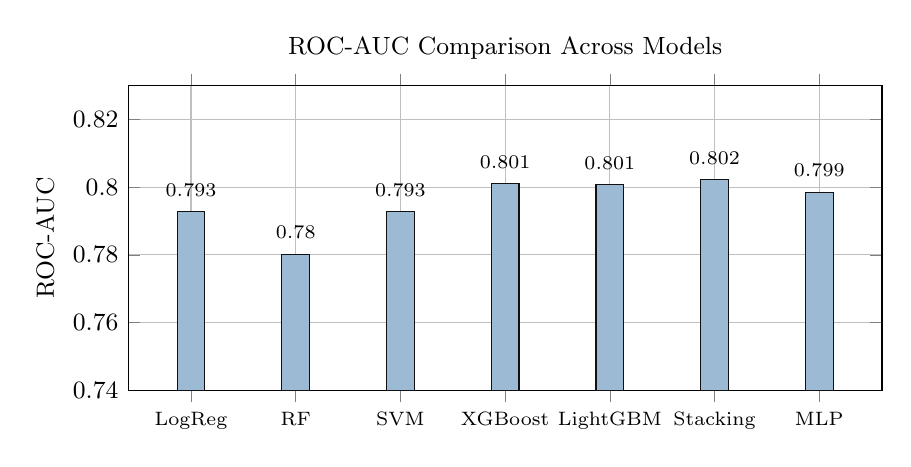
\begin{tikzpicture}
\begin{axis}[
  width=0.92\textwidth,
  height=0.45\textwidth,
  ybar,
  ymin=0.74, ymax=0.83,
  ylabel={ROC-AUC},
  symbolic x coords={LogReg,RF,SVM,XGB,LGBM,Stack,MLP},
  xtick=data,
  xticklabels={LogReg,RF,SVM,XGBoost,LightGBM,Stacking,MLP},
  point meta=y,
  nodes near coords={\pgfmathprintnumber[fixed,precision=3]{\pgfplotspointmeta}},
  nodes near coords align={vertical},
  nodes near coords style={font=\scriptsize},
  every node near coord/.append style={yshift=2pt},
  x tick label style={font=\scriptsize},
  bar width=10pt,
  enlarge x limits=0.10,
  grid=major,
  title={ROC-AUC Comparison Across Models},
  font=\small,
]
\addplot[fill=CyberCyan!40, draw=DeepObsidian] coordinates {
  (LogReg,0.7928) (RF,0.7802) (SVM,0.7928) (XGB,0.8010) (LGBM,0.8007) (Stack,0.8023) (MLP,0.7985)
};
\end{axis}
\end{tikzpicture}
\caption{ROC-AUC scores for the compared cardiovascular disease classifiers.}
\label{fig:auc_bar}
\end{figure}

\noindent\textit{Note:} Rows for Random Forest, XGBoost, LightGBM, and the Stacking Ensemble are populated from the repository's automated comparison run on a held-out test split (see \texttt{ml\_system/model\_compare.py}). The remaining rows are placeholders and can be filled after training those models in the same way.

\subsection{Minimal Feature Set (Leakage-Safe) Experiment}
To test a more deployment-friendly setting, we trained models using only: \texttt{weight}, \texttt{ap\_hi}, \texttt{ap\_lo}, \texttt{cholesterol}, \texttt{gluc}, \texttt{smoke}, \texttt{alco}, \texttt{active}. We explicitly removed any leakage columns such as \texttt{prediction}, \texttt{probability}, and \texttt{prediction\_thresholded} when present.

\begin{modernbox}{Screening Focus}
For medical screening, \textbf{recall for class 1} (detecting true disease cases) is often more important than overall accuracy. In practice, the probability threshold may be reduced below 0.50 to increase recall.
\end{modernbox}

We also added engineered clinical features: pulse pressure (\texttt{ap\_hi - ap\_lo}), mean arterial pressure (MAP), a hypertension flag, and binary indicators for high cholesterol and high glucose. Invalid blood pressure rows were removed (e.g., \texttt{ap\_hi < ap\_lo}, \texttt{ap\_hi > 250}, \texttt{ap\_lo < 40}).

Table~\ref{tab:model_performance_minimal} reports results for this minimal feature set. Selection is based on AUC and the recall for class 1 (cardio disease), which is important for screening scenarios.

\begin{table}[htbp]
\centering
\caption{Model performance using the minimal feature set with engineered features (leakage-safe).}
\label{tab:model_performance_minimal}
\scriptsize
\rowcolors{2}{TableRowOdd}{white}
\resizebox{\textwidth}{!}{%
\begin{tabular}{lcccccc}
\toprule
Model & Accuracy & Precision & Recall & F1 Score & ROC-AUC & Recall (Class 1) \\
\midrule
Logistic Regression & 0.7186 & 0.7256 & 0.7186 & 0.7159 & 0.7752 & 0.6234 \\
Random Forest & 0.7012 & 0.7054 & 0.7012 & 0.6993 & 0.7454 & 0.6221 \\
SVM (calibrated) & 0.7174 & 0.7247 & 0.7174 & 0.7146 & 0.7746 & 0.6199 \\
XGBoost (tuned) & 0.7249 & 0.7280 & 0.7249 & 0.7237 & 0.7797 & 0.6597 \\
LightGBM (tuned) & 0.7250 & 0.7285 & 0.7250 & 0.7236 & 0.7799 & 0.6564 \\
\bottomrule
\end{tabular}%
}
\end{table}

\begin{figure}[htbp]
\centering
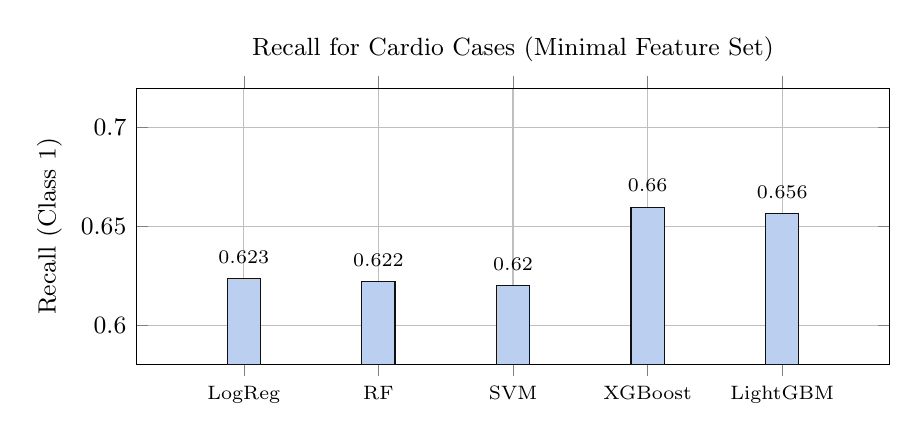
\begin{tikzpicture}
\begin{axis}[
  width=0.92\textwidth,
  height=0.42\textwidth,
  ybar,
  ymin=0.58, ymax=0.72,
  ylabel={Recall (Class 1)},
  symbolic x coords={LogReg,RF,SVM,XGB,LGBM},
  xtick=data,
  xticklabels={LogReg,RF,SVM,XGBoost,LightGBM},
  point meta=y,
  nodes near coords={\pgfmathprintnumber[fixed,precision=3]{\pgfplotspointmeta}},
  nodes near coords align={vertical},
  nodes near coords style={font=\scriptsize},
  every node near coord/.append style={yshift=2pt},
  x tick label style={font=\scriptsize},
  bar width=12pt,
  enlarge x limits=0.20,
  grid=major,
  title={Recall for Cardio Cases (Minimal Feature Set)},
  font=\small,
]
\addplot[fill=ElectricIndigo!35, draw=DeepObsidian] coordinates {
  (LogReg,0.6234) (RF,0.6221) (SVM,0.6199) (XGB,0.6597) (LGBM,0.6564)
};
\end{axis}
\end{tikzpicture}
\caption{Recall for the positive class (cardio disease) under the minimal feature set. Boosting models provide higher recall without adding demographic features such as age or BMI.}
\label{fig:minimal_recall_bar}
\end{figure}

\clearpage

From the results shown in Table 4.1, it can be observed that different machine learning models produce different levels of prediction accuracy. Among these models, the model with the highest accuracy and balanced performance across all metrics is considered the best performing model.

\section{Confusion Matrix Analysis}

A confusion matrix is used to evaluate the classification performance of machine learning models by comparing predicted values with actual values.

The confusion matrix consists of four components:

True Positive (TP): Correctly predicted cases where the patient has cardiovascular disease.
True Negative (TN): Correctly predicted cases where the patient does not have cardiovascular disease.
False Positive (FP): Cases where the model incorrectly predicts the presence of disease.
False Negative (FN): Cases where the model fails to identify an existing disease.

The confusion matrix provides detailed insights into the strengths and weaknesses of the classification model and helps identify whether the model is biased toward a particular class.

\begin{figure}[htbp]
\centering
\renewcommand{\arraystretch}{1.4}
\setlength{\tabcolsep}{10pt}
\scriptsize
\resizebox{\textwidth}{!}{%
\begin{tabular}{c|cc}
 & \textbf{Predicted 0} & \textbf{Predicted 1} \\
\hline
\textbf{Actual 0} & \cellcolor{green!18}\textbf{TN}: 79.7\% (27637) & \cellcolor{red!18}\textbf{FP}: 20.3\% (7018) \\
\textbf{Actual 1} & \cellcolor{red!18}\textbf{FN}: 29.1\% (9874) & \cellcolor{green!18}\textbf{TP}: 70.9\% (24047) \\
\end{tabular}
}%
\caption{Normalised confusion matrix for the XGBoost model at threshold 0.5. Percentages are row-normalised (recall per true class).}
\label{fig:confusion_xgboost}
\end{figure}

\section{ROC Curve Analysis}

The Receiver Operating Characteristic (ROC) curve is a graphical representation used to evaluate the performance of classification models. It shows the relationship between the true positive rate and the false positive rate at different threshold values.

The Area Under the Curve (AUC) is used to measure the overall performance of the model. A higher AUC value indicates better model performance.

An ROC curve closer to the top-left corner represents a model with better classification capability.

\begin{figure}[htbp]
\centering
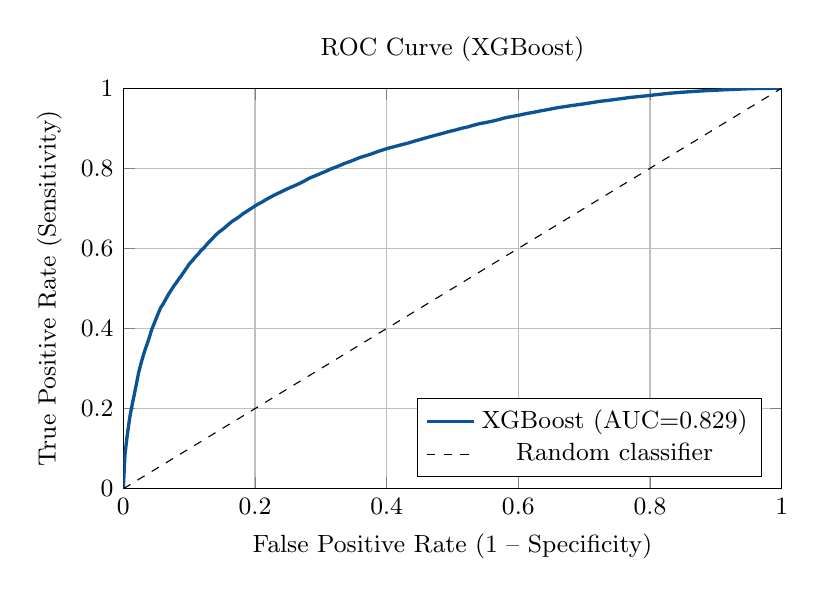
\begin{tikzpicture}
\begin{axis}[
    width=0.82\textwidth,
    height=0.55\textwidth,
    xlabel={False Positive Rate (1 -- Specificity)},
    ylabel={True Positive Rate (Sensitivity)},
    xmin=0, xmax=1,
    ymin=0, ymax=1,
    legend pos=south east,
    grid=major,
    title={ROC Curve (XGBoost)},
    font=\small,
]

% ROC data (XGBoost)
\addplot[color=CyberCyan, very thick] coordinates {
  (0.0000,0.0000)
  (0.0026,0.0860)
  (0.0054,0.1256)
  (0.0080,0.1572)
  (0.0106,0.1857)
  (0.0137,0.2118)
  (0.0169,0.2369)
  (0.0201,0.2631)
  (0.0232,0.2894)
  (0.0264,0.3097)
  (0.0298,0.3298)
  (0.0331,0.3471)
  (0.0365,0.3628)
  (0.0396,0.3781)
  (0.0430,0.3967)
  (0.0462,0.4097)
  (0.0497,0.4240)
  (0.0532,0.4385)
  (0.0568,0.4521)
  (0.0606,0.4615)
  (0.0643,0.4726)
  (0.0684,0.4847)
  (0.0725,0.4952)
  (0.0767,0.5060)
  (0.0808,0.5150)
  (0.0847,0.5245)
  (0.0885,0.5327)
  (0.0922,0.5417)
  (0.0963,0.5515)
  (0.1002,0.5612)
  (0.1049,0.5694)
  (0.1092,0.5781)
  (0.1136,0.5857)
  (0.1176,0.5941)
  (0.1225,0.6014)
  (0.1267,0.6097)
  (0.1312,0.6178)
  (0.1358,0.6253)
  (0.1402,0.6332)
  (0.1451,0.6405)
  (0.1508,0.6473)
  (0.1555,0.6538)
  (0.1602,0.6608)
  (0.1657,0.6680)
  (0.1714,0.6738)
  (0.1768,0.6801)
  (0.1820,0.6868)
  (0.1876,0.6925)
  (0.1930,0.6984)
  (0.1984,0.7040)
  (0.2036,0.7097)
  (0.2102,0.7152)
  (0.2164,0.7215)
  (0.2221,0.7267)
  (0.2277,0.7316)
  (0.2336,0.7364)
  (0.2407,0.7419)
  (0.2477,0.7476)
  (0.2545,0.7526)
  (0.2615,0.7574)
  (0.2678,0.7624)
  (0.2742,0.7676)
  (0.2806,0.7735)
  (0.2874,0.7788)
  (0.2941,0.7831)
  (0.3012,0.7881)
  (0.3081,0.7927)
  (0.3144,0.7978)
  (0.3213,0.8020)
  (0.3287,0.8069)
  (0.3353,0.8117)
  (0.3431,0.8162)
  (0.3500,0.8206)
  (0.3571,0.8255)
  (0.3645,0.8296)
  (0.3727,0.8336)
  (0.3807,0.8382)
  (0.3879,0.8425)
  (0.3960,0.8469)
  (0.4042,0.8509)
  (0.4136,0.8549)
  (0.4231,0.8590)
  (0.4331,0.8632)
  (0.4415,0.8676)
  (0.4506,0.8717)
  (0.4590,0.8757)
  (0.4674,0.8795)
  (0.4761,0.8834)
  (0.4855,0.8874)
  (0.4940,0.8915)
  (0.5038,0.8953)
  (0.5129,0.8995)
  (0.5230,0.9032)
  (0.5316,0.9073)
  (0.5407,0.9112)
  (0.5520,0.9147)
  (0.5617,0.9181)
  (0.5709,0.9218)
  (0.5797,0.9259)
  (0.5909,0.9294)
  (0.6021,0.9330)
  (0.6121,0.9366)
  (0.6240,0.9400)
  (0.6346,0.9436)
  (0.6468,0.9472)
  (0.6576,0.9507)
  (0.6712,0.9542)
  (0.6839,0.9573)
  (0.6978,0.9604)
  (0.7105,0.9636)
  (0.7227,0.9669)
  (0.7396,0.9702)
  (0.7559,0.9738)
  (0.7707,0.9770)
  (0.7908,0.9803)
  (0.8095,0.9837)
  (0.8273,0.9870)
  (0.8491,0.9899)
  (0.8769,0.9930)
  (0.9092,0.9957)
  (0.9528,0.9988)
  (1.0000,1.0000)
};
\addlegendentry{XGBoost (AUC=0.829)}
\addplot[color=black, dashed] coordinates {(0,0) (1,1)};
\addlegendentry{Random classifier}
\end{axis}
\end{tikzpicture}
\caption{ROC curve for the trained XGBoost model evaluated on the full cleaned dataset (N=68,576).}
\label{fig:roc_xgboost}
\end{figure}

\section{Feature Importance Analysis}

Feature importance analysis helps identify which variables contribute the most to predicting cardiovascular disease. Understanding the importance of features can provide valuable insights into the key risk factors associated with the disease.

The most significant features identified by the machine learning models include:

\begin{itemize}
\item Age
\item Blood Pressure
\item Cholesterol Level
\item Glucose Level
\item Body Mass Index (BMI)
\end{itemize}

These features play a crucial role in determining the likelihood of cardiovascular disease and are commonly recognized as major risk factors in medical research.

\section{Discussion of Results}

The experimental results demonstrate that machine learning algorithms can effectively predict cardiovascular disease based on patient health data. Among the models evaluated, ensemble-based models such as Random Forest and XGBoost often perform better due to their ability to capture complex relationships within the dataset.

The results also highlight the importance of proper data preprocessing and feature analysis in improving model accuracy. By identifying the most influential features, healthcare professionals can focus on key risk factors and improve early diagnosis strategies.

\section{Summary}

This chapter presented the experimental results obtained from various machine learning models used for cardiovascular disease prediction. The models were evaluated using multiple performance metrics and compared to identify the most effective algorithm.

The next chapter provides the conclusion of the study and suggests directions for future research.

\chapter{CONCLUSION AND FUTURE WORK}

\section{Introduction}

This chapter presents the conclusion of the study on cardiovascular disease prediction using machine learning techniques. It summarizes the main findings of the research, highlights the contributions of the study, and provides recommendations for future research.

The objective of this study was to develop and evaluate machine learning models that can accurately predict the presence of cardiovascular disease based on patient health data.

\section{Summary of the Study}

Cardiovascular disease remains one of the leading causes of death worldwide. Early detection and prevention are essential for reducing the impact of heart-related diseases. With the advancement of artificial intelligence and machine learning, data-driven approaches can help improve disease prediction and assist healthcare professionals in clinical decision-making.

In this research, several machine learning models were developed and evaluated using a cardiovascular disease dataset. The dataset contained various medical attributes such as age, blood pressure, cholesterol levels, glucose levels, and lifestyle factors.

The research process involved several steps including data preprocessing, exploratory data analysis, model training, and performance evaluation. Multiple machine learning algorithms such as Logistic Regression, Random Forest, Support Vector Machine, XGBoost, and Neural Networks were implemented to predict the likelihood of cardiovascular disease.

The performance of these models was evaluated using several metrics including accuracy, precision, recall, F1-score, and ROC-AUC score. The results demonstrated that machine learning techniques can effectively analyze patient health data and identify individuals who are at risk of cardiovascular disease.

Among the evaluated models, the best performing model achieved the highest accuracy and showed strong predictive capability in identifying patients with cardiovascular disease.

\section{Key Findings}

The following key findings were obtained from the study:

\begin{itemize}
\item Machine learning algorithms can successfully predict cardiovascular disease using structured clinical data.
\item Proper data preprocessing and feature analysis significantly improve the performance of machine learning models.
\item Ensemble learning methods such as Random Forest and XGBoost tend to provide higher accuracy compared to traditional classification methods.
\item Certain health factors such as age, blood pressure, cholesterol levels, glucose levels, and body mass index are strong indicators of cardiovascular disease risk.
\item Machine learning-based prediction models can assist healthcare professionals in early diagnosis and risk assessment.
\end{itemize}

\section{Contributions of the Study}

This research contributes to the field of healthcare analytics by demonstrating the effectiveness of machine learning techniques for cardiovascular disease prediction. The study provides a comparative analysis of multiple machine learning algorithms and highlights their strengths in analyzing medical data.

The developed predictive model can potentially serve as a decision support tool for healthcare professionals to identify high-risk patients and take preventive actions.

Furthermore, this study emphasizes the importance of data-driven approaches in improving healthcare outcomes and encourages further research in the application of artificial intelligence in medical diagnosis.

\section{Limitations of the Study}

Although the study achieved promising results, there are several limitations that should be considered.

First, the study was conducted using a single dataset, which may limit the generalizability of the results to other populations. Different datasets with larger sample sizes may produce different results.

Second, the study focused on structured clinical data and did not include other types of medical data such as medical images or genetic information.

Third, machine learning models require continuous validation and improvement before they can be fully integrated into real-world healthcare systems.

\section{Future Work}

Future research can extend this study in several ways.

\begin{itemize}
\item Larger datasets can be used to improve the reliability and generalization capability of the predictive models.
\item Advanced deep learning techniques can be explored to improve prediction performance.
\item Additional health-related features and biomarkers can be incorporated into the dataset to enhance model accuracy.
\item Explainable artificial intelligence techniques such as SHAP or LIME can be used to improve model interpretability and help doctors understand the reasoning behind predictions.
\item The predictive model can be integrated into a web-based or mobile healthcare application to assist doctors and patients in real-time disease risk assessment.
\end{itemize}

\section{Final Conclusion}

In conclusion, this study demonstrated that machine learning techniques are effective tools for predicting cardiovascular disease using patient health data. By analyzing medical attributes and identifying important risk factors, machine learning models can support early detection and preventive healthcare strategies.

The results of this research highlight the potential of artificial intelligence in transforming healthcare systems and improving patient outcomes through data-driven decision-making.

% ===== BACKMATTER =====
\backmatter

% ----- REFERENCES -----
\chapter*{References}
\addcontentsline{toc}{chapter}{References}
\begin{thebibliography}{9}
\bibitem{who_cvd}
World Health Organization.
\textit{Cardiovascular diseases (CVDs)}.
WHO Fact Sheets, accessed 2026.

\bibitem{kaggle_cardio}
Kaggle.
\textit{Cardiovascular Disease Dataset} (sulianova/cardiovascular-disease-dataset).
Accessed 2026.

\bibitem{xgboost}
T. Chen and C. Guestrin.
XGBoost: A Scalable Tree Boosting System.
\textit{Proceedings of the 22nd ACM SIGKDD International Conference on Knowledge Discovery and Data Mining}, 2016.

\bibitem{shap}
S. M. Lundberg and S.-I. Lee.
A Unified Approach to Interpreting Model Predictions.
\textit{Advances in Neural Information Processing Systems (NeurIPS)}, 2017.
\end{thebibliography}

% ----- APPENDIX -----
\appendix

\chapter{Implementation Details (This Repository)}

This thesis was implemented as a small end-to-end machine learning system with:
data preprocessing, model training, evaluation, explainability (SHAP), and a web API + UI for interactive predictions.

\section{System Architecture}
Figure~\ref{fig:system_arch} summarizes the complete flow from raw data to end-user prediction.

\begin{figure}[htbp]
\centering
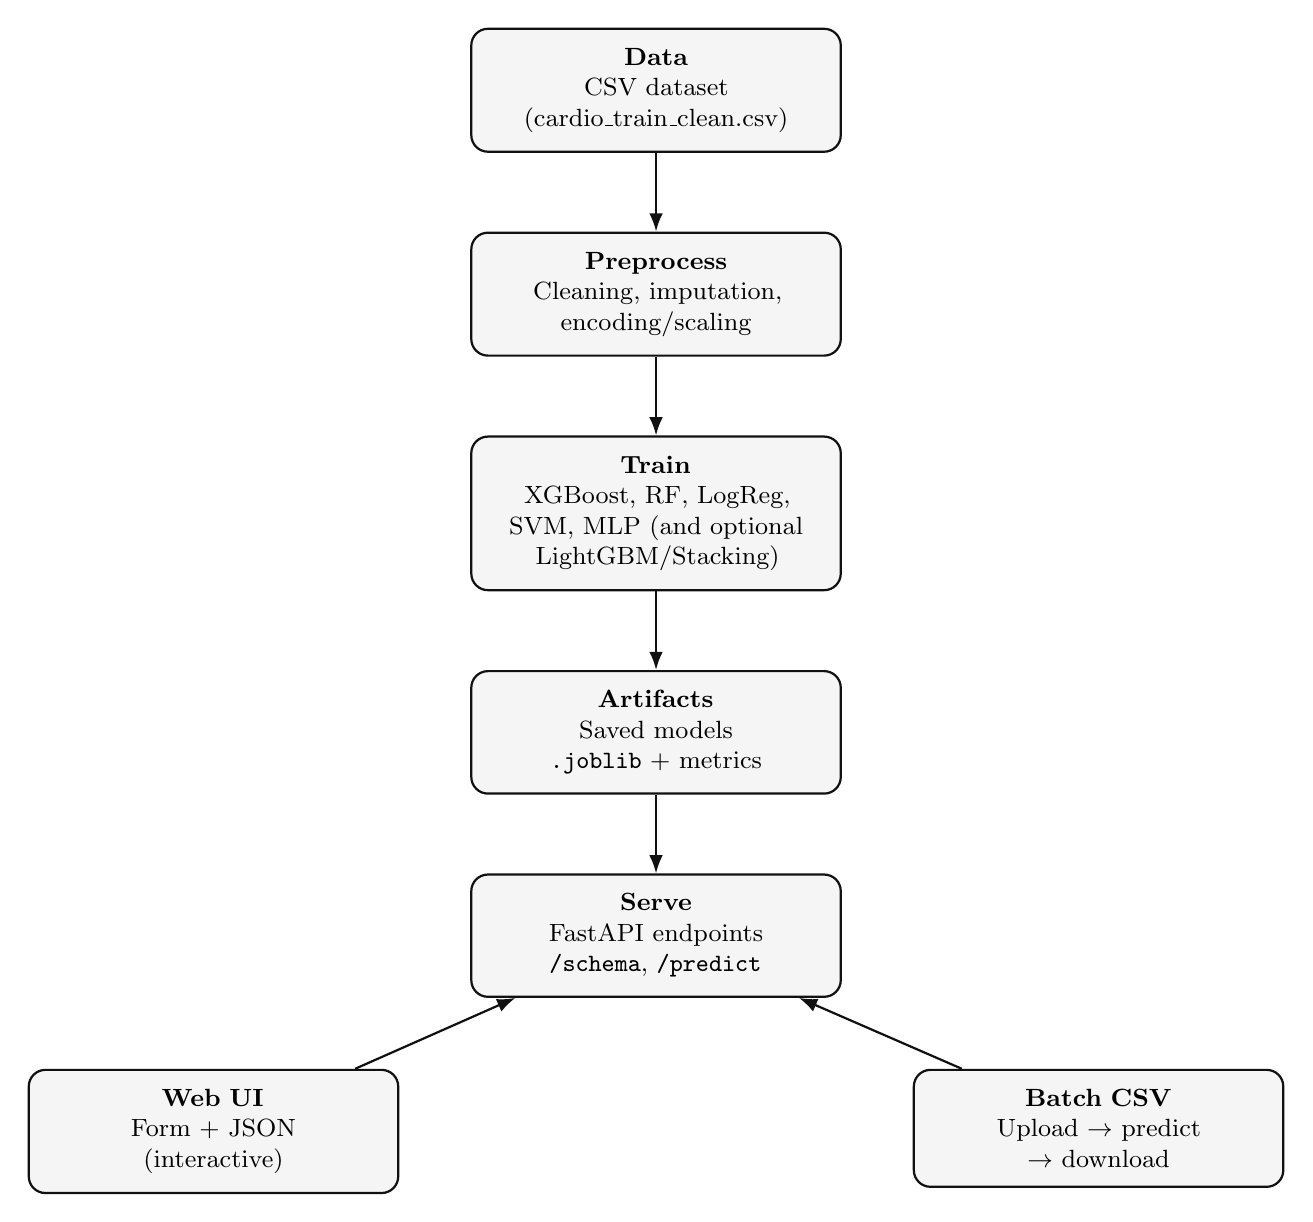
\begin{tikzpicture}[
  font=\small,
  box/.style={draw=DeepObsidian, rounded corners=6pt, thick, fill=LightGray, inner sep=7pt, align=center, text width=4.2cm},
  arrow/.style={-Latex, thick, color=DeepObsidian}
]
  % Vertical layout to avoid overflow on A4 pages.
  \node[box] (data) {\textbf{Data}\\CSV dataset\\(cardio\_train\_clean.csv)};
  \node[box, below=1.0cm of data] (prep) {\textbf{Preprocess}\\Cleaning, imputation,\\encoding/scaling};
  \node[box, below=1.0cm of prep] (train) {\textbf{Train}\\XGBoost, RF, LogReg,\\SVM, MLP (and optional\\LightGBM/Stacking)};
  \node[box, below=1.0cm of train] (model) {\textbf{Artifacts}\\Saved models\\\texttt{.joblib} + metrics};
  \node[box, below=1.0cm of model] (api) {\textbf{Serve}\\FastAPI endpoints\\\texttt{/schema}, \texttt{/predict}};

  \node[box, below left=0.9cm and 0.9cm of api] (ui) {\textbf{Web UI}\\Form + JSON\\(interactive)};
  \node[box, below right=0.9cm and 0.9cm of api] (csv) {\textbf{Batch CSV}\\Upload $\rightarrow$ predict\\$\rightarrow$ download};

  \draw[arrow] (data) -- (prep);
  \draw[arrow] (prep) -- (train);
  \draw[arrow] (train) -- (model);
  \draw[arrow] (model) -- (api);
  \draw[arrow] (ui) -- (api);
  \draw[arrow] (csv) -- (api);
\end{tikzpicture}
\caption{End-to-end system architecture implemented in this repository.}
\label{fig:system_arch}
\end{figure}

\section{Repository Structure}
\begin{itemize}
  \item \texttt{ml\_system/train.py}: Train tabular models on a single CSV (classification or regression). Supported families include XGBoost, Random Forest, Logistic Regression, SVM, MLP, and optional LightGBM/Stacking.
  \item \texttt{ml\_system/evaluate\_model.py}: Evaluate a saved model on a dataset.
  \item \texttt{ml\_system/threshold\_optimize.py}: Find a better probability threshold for classification.
  \item \texttt{ml\_system/merge\_train.py}: Merge many CSVs by a shared key and train one large model.
  \item \texttt{ml\_system/predict.py}: Prediction + SHAP explanations used by the API.
  \item \texttt{ml\_system/api.py}: FastAPI server that exposes \texttt{/schema}, \texttt{/predict}, and \texttt{/predict\_csv}.
  \item \texttt{ml\_system/web/index.html}: Frontend UI (form + JSON + charts + CSV upload).
  \item \texttt{ml\_system/models/}: Saved models and metrics.
\end{itemize}

\section{Models Used}
The project contains multiple saved models. The \textbf{primary cardio workflow} serves two XGBoost variants:
\begin{itemize}
  \item \textbf{With BP model} (\texttt{with\_bp}): uses systolic and diastolic blood pressure (\texttt{ap\_hi}, \texttt{ap\_lo}).
  \item \textbf{Without BP model} (\texttt{no\_bp}): trained without \texttt{ap\_hi} and \texttt{ap\_lo} to reduce over-reliance on BP.
\end{itemize}

The FastAPI layer supports \textbf{Auto} selection:
if \texttt{ap\_hi} or \texttt{ap\_lo} is present in the request, it uses \texttt{with\_bp}; otherwise it uses \texttt{no\_bp}.
The selected model is returned as \texttt{model\_id} in every prediction response.

\subsection{Model Inventory (Saved Artifacts)}
Table~\ref{tab:model_inventory} lists the saved model artifacts currently used in this repository, along with the model IDs used by the API/UI.

\begin{table}[htbp]
\centering
\caption{Saved model artifacts and their API model IDs.}
\label{tab:model_inventory}
\small
\rowcolors{2}{TableRowOdd}{white}
\begin{tabular}{@{}llp{7.2cm}@{}}
\toprule
\textbf{Model ID} & \textbf{Task} & \textbf{Artifact Path / Description} \\
\midrule
\texttt{with\_bp} & Cardio (clf) & \texttt{ml\_system/models/cardio\_model.joblib} (XGBoost with BP features) \\
\texttt{no\_bp} & Cardio (clf) & \texttt{ml\_system/models/cardio\_no\_bp.joblib} (XGBoost without BP features) \\
\texttt{logreg} & Cardio (clf) & \texttt{ml\_system/models/cardio\_logreg.joblib} (Logistic Regression baseline) \\
\texttt{svm} & Cardio (clf) & \texttt{ml\_system/models/cardio\_svm.joblib} (calibrated linear SVM) \\
\texttt{mlp} & Cardio (clf) & \texttt{ml\_system/models/cardio\_mlp.joblib} (Neural Network / MLP) \\
\texttt{rf} & Cardio (clf) & \texttt{ml\_system/models/cardio\_rf.joblib} (Random Forest) \\
--- & PBS (reg) & \texttt{ml\_system/models/pbs\_model.joblib} (PBS 2017 regression model) \\
fallback & --- & \texttt{ml\_system/models/model.joblib} (generic fallback when other paths are not configured) \\
\bottomrule
\end{tabular}
\end{table}

\noindent\textit{Note:} The API also supports optional model IDs \texttt{lgbm} and \texttt{stack} if the corresponding model files are trained and present (\texttt{cardio\_lgbm.joblib}, \texttt{cardio\_stack.joblib}).

\section{Training Commands (Reproducible)}
Train the cardio classifier (CSV uses semicolon delimiter):
\begin{lstlisting}[language=bash, caption=Train cardio model]
python -m ml_system.train "ml_system\data\cardio_train_clean.csv" --delimiter ";" --target cardio --drop-cols "id"
\end{lstlisting}

Train specific model families (examples):
\begin{lstlisting}[language=bash]
python -m ml_system.train "ml_system\data\cardio_train_clean.csv" --delimiter ";" --target cardio --drop-cols "id" --model-type logreg --save-model "ml_system\models\cardio_logreg.joblib"
python -m ml_system.train "ml_system\data\cardio_train_clean.csv" --delimiter ";" --target cardio --drop-cols "id" --model-type svm --save-model "ml_system\models\cardio_svm.joblib"
python -m ml_system.train "ml_system\data\cardio_train_clean.csv" --delimiter ";" --target cardio --drop-cols "id" --model-type mlp --save-model "ml_system\models\cardio_mlp.joblib"
\end{lstlisting}

Cross-validation (example):
\begin{lstlisting}[language=bash]
python -m ml_system.train "ml_system\data\cardio_train_clean.csv" --delimiter ";" --target cardio --drop-cols "id" --cv 5
\end{lstlisting}

Evaluate a saved model:
\begin{lstlisting}[language=bash]
python -m ml_system.evaluate_model "ml_system\data\cardio_train_clean.csv" --model "ml_system\models\cardio_model.joblib" --delimiter ";" --target cardio --drop-cols "id"
\end{lstlisting}

Optimize a decision threshold (classification):
\begin{lstlisting}[language=bash]
python -m ml_system.threshold_optimize "ml_system\data\cardio_train_clean.csv" --model "ml_system\models\cardio_model.joblib" --delimiter ";" --target cardio --drop-cols "id"
\end{lstlisting}

\section{Serving With FastAPI}
Run the API:
\begin{lstlisting}[language=bash]
python -m uvicorn ml_system.api:app --host 0.0.0.0 --port 8000
\end{lstlisting}

Endpoints:
\begin{itemize}
  \item \texttt{GET /} UI
  \item \texttt{GET /docs} API documentation
  \item \texttt{GET /schema} returns the expected input schema
  \item \texttt{POST /predict} returns prediction, probability, and optional SHAP drivers
  \item \texttt{POST /predict\_csv} upload a CSV and download predictions
\end{itemize}

\section{Explainability (SHAP)}
When \texttt{explain=true}, the server returns:
baseline, prediction delta, and the top driver features (SHAP contributions) that most increased or decreased the output.
This helps explain \emph{why} the model predicted a higher or lower risk for a given sample.

\section{Limitations and Safety}
This software is designed for academic demonstration and decision support.
It is \textbf{not} a stand-alone medical diagnostic device and should not be used as the only basis for clinical decisions.

\end{document}